\documentclass{beamer}
\usepackage{pgfpages}
%\setbeameroption{show notes on second screen=left} %enable for notes
\usepackage{graphicx}
\usepackage{xcolor}
\usepackage{listings}
\usepackage{hyperref}
\lstset{language=python,frame=single}
\usepackage{verbatim}
%\usepackage{apacite}
\usepackage{natbib}
\usepackage{subcaption}
\usepackage{amsmath}
\usepackage{relsize}
\usepackage{appendixnumberbeamer}
\usepackage{xparse}
\usepackage{multimedia}
\usepackage{xcolor}
\usepackage[normalem]{ulem}
\usepackage{tikz}
\usetikzlibrary{matrix,backgrounds}
\usetikzlibrary{positioning}
\pgfdeclarelayer{myback}
\pgfsetlayers{myback,background,main}

\tikzset{
  invisible/.style={opacity=0},
  visible on/.style={alt={#1{}{invisible}}},
  alt/.code args={<#1>#2#3}{%
    \alt<#1>{\pgfkeysalso{#2}}{\pgfkeysalso{#3}} % \pgfkeysalso doesn't change the path
  },
}
\tikzset{fontscale/.style = {font=\relsize{#1}}}
\tikzset{mycolor/.style = {line width=1bp,color=#1}}%
\tikzset{myfillcolor/.style = {draw,fill=#1}}%
\tikzset{ 
    table/.style={
        matrix of nodes,
        row sep=-\pgflinewidth,
        column sep=-\pgflinewidth,
        nodes={
            rectangle,
            draw=black,
            align=center,
	    fill=gray!10
        },
        minimum height=1em,
        text depth=0.1ex,
        text height=1ex,
	text width=0.6em,
	fontscale=-4,
        nodes in empty cells
    }
}
\def\myletdropspace{0.05cm}

\NewDocumentCommand{\highlight}{O{blue!40} m m}{%
\draw[mycolor=#1,rounded corners] (#2.north west)rectangle (#3.south east);
}

\NewDocumentCommand{\fhighlight}{O{blue!40} m m}{%
\draw[myfillcolor=#1,rounded corners] (#2.north west)rectangle (#3.south east);
}

\usetheme[numbering=fraction]{metropolis}
%%\AtBeginSection[]
%%{
%%  \begin{frame}
%%    \frametitle{Table of Contents}
%%    \tableofcontents[currentsection]
%%  \end{frame}
%%}

%%\let\olditem\item
%%\renewcommand{\item}{\vspace{0.5\baselineskip}\olditem}
\begin{document}

\title{The Jabberwocky}
\subtitle{One-shot and few-shot learning of word embeddings}
\author{Andrew Lampinen}
\date{CSLI, 9/12/2017}
\frame{\titlepage}

\begin{frame}{One-shot word learning}
\begin{columns}
\begin{column}{0.5\textwidth}
\textit{’Twas brillig, and the slithy toves}\\
\textit{Did gyre and gimble in the wabe:}\\ 
\textit{All mimsy were the borogoves,}\\
\textit{And the mome raths outgrabe.}\\[10pt]

\textit{“Beware the Jabberwock, my son! }\\
\textit{The jaws that bite, the claws that catch!}\\
\textit{Beware the Jubjub bird, and shun}\\ 
\textit{The frumious Bandersnatch!” }\\[10pt]

\textit{He took his vorpal sword in hand}\\
\textit{[...]}
\end{column}
\begin{column}{0.5\textwidth}
\centering
\includegraphics[height=0.8\textheight]{figures/Jabberwocky.jpg}
\end{column}
\end{columns}
\end{frame}

\begin{frame}{Introduction}
One-shot learning of word embeddings? 
\begin{itemize}
    \item<2-> Word-embedding based systems are achieving quite good performance on some tasks. 
    \item<3-> But humans can learn fast.
    \item<4-> Can CLS resolve this?
\end{itemize}
\end{frame}

\begin{frame}{One-shot word learning}
We'll look at this in the context of prediction:\\[11pt]
\begin{figure}
\centering
\begin{tikzpicture}
\node (w1) [visible on=<1->] {He};
\node (w2) [right=1.6cm of w1.center, anchor=center, visible on=<1->] {took};
\node (w3) [right=1.6cm of w2.center, anchor=center, visible on=<1->] {his};
\node (w4) [below right=\myletdropspace and 1.6cm of w3.center, anchor=center, visible on=<1->] {
    \only<-3>{vorpal}
    \only<4->{\textcolor{red}{vorpal}}
};
\node (w5) [above right=\myletdropspace and 1.6cm of w4.center, anchor=center, visible on=<1->] {sword};
\node (w6) [right=1.6cm of w5.center, anchor=center, visible on=<1->] {in};
\node (w7) [right=1.6cm of w6.center, anchor=center, visible on=<1->] {hand};

\node (n1) [draw, above=0.75cm of w1, visible on=<1->] {?};
\node (n2) [draw, above=0.75cm of w2, visible on=<2->] {?};
\node (n3) [draw, above=0.75cm of w3, visible on=<3->] {?};
\node (n4) [draw, above=0.76cm of w4, visible on=<4->] {?};
\node (n5) [draw, above=0.75cm of w5, visible on=<5->] {?};
\node (n6) [draw, above=0.75cm of w6, visible on=<6->] {?};
\node (n7) [draw, above=0.75cm of w7, visible on=<7->] {?};

\node (ow1) [above=0.75cm of n1, visible on=<1->] {took};
\node (ow2) [above=0.75cm of n2, visible on=<2->] {his};
\node (ow3) [above=0.7cm of n3, visible on=<3->, align=center] {
    \only<3>{sharp}
    \only<4->{\textcolor{red}{vorpal}\\\sout{sharp}}
};
\node (ow4) [above=0.75cm of n4, visible on=<4->] {sword};
\node (ow5) [above=0.75cm of n5, visible on=<5->] {in};
\node (ow6) [above=0.75cm of n6, visible on=<6->] {hand};
\node (ow7) [above=0.75cm of n7, visible on=<7->] {,};

\draw [->, visible on=<1->] (w1) -- (n1);
\draw [->, visible on=<2->] (w2) -- (n2);
\draw [->, visible on=<3->] (w3) -- (n3);
\draw [->, visible on=<4->] (w4) -- (n4);
\draw [->, visible on=<5->] (w5) -- (n5);
\draw [->, visible on=<6->] (w6) -- (n6);
\draw [->, visible on=<7->] (w7) -- (n7);

\draw [->, visible on=<1->] (n1) -- (ow1);
\draw [->, visible on=<2->] (n2) -- (ow2);
\draw [->, visible on=<3->] (n3) -- (ow3);
\draw [->, visible on=<4->] (n4) -- (ow4);
\draw [->, visible on=<5->] (n5) -- (ow5);
\draw [->, visible on=<6->] (n6) -- (ow6);
\draw [->, visible on=<7->] (n7) -- (ow7);

\draw [->, visible on=<2->] (n1) -- (n2);
\draw [->, visible on=<3->] (n2) -- (n3);
\draw [->, visible on=<4->] (n3) -- (n4);
\draw [->, visible on=<5->] (n4) -- (n5);
\draw [->, visible on=<6->] (n5) -- (n6);
\draw [->, visible on=<7->] (n6) -- (n7);
\end{tikzpicture}
\end{figure}
\end{frame}

\begin{frame}<1>[label=netdiagram]
\frametitle{One-shot word learning}
\only<1>{Using model from \citet{Zaremba2014a}.\\[-15pt]}
\begin{figure}
\centering
\begin{tikzpicture}[ampersand replacement=\&]
\node (w1) [visible on=<1->] {He};
\node (w2) [right=1.6cm of w1.center, anchor=center] {took};
\node (w3) [right=1.6cm of w2.center, anchor=center] {his};
\node (w4) [below right=\myletdropspace and 1.6cm of w3.center, anchor=center] {
    \textcolor{red}{vorpal}
};
\node (w5) [above right=\myletdropspace and 1.6cm of w4.center, anchor=center] {sword};
\node (w6) [right=1.6cm of w5.center, anchor=center] {in};
\node (w7) [right=1.6cm of w6.center, anchor=center] {hand};

\matrix (v1) [table, above=0.75cm of w1] {
0.2 \& 0.7 \& \dots \\
};
\matrix (v2) [table, above=0.75cm of w2] {
0.5 \& 2.0 \& \dots \\ 
};
\matrix (v3) [table, above=0.75cm of w3] {
0.1\& 0.2 \& \dots \\ 
};
\matrix (v4) [table, above=0.77cm of w4, text=red] {
? \& ? \& \dots \\ 
};
\matrix (v5) [table, above=0.75cm of w5] {
5.1 \& 0.1 \& \dots \\ 
};
\matrix (v6) [table, above=0.75cm of w6] {
0.9 \& 0.6 \& \dots \\ 
};
\matrix (v7) [table, above=0.75cm of w7] {
0.3 \& 0.0 \& \dots \\ 
};

\node (n1) [draw, above=0.5cm of v1, fontscale=-2] {LSTM};
\node (n2) [draw, above=0.5cm of v2, fontscale=-2] {LSTM};
\node (n3) [draw, above=0.5cm of v3, fontscale=-2] {LSTM};
\node (n4) [draw, above=0.5cm of v4, fontscale=-2] {LSTM};
\node (n5) [draw, above=0.5cm of v5, fontscale=-2] {LSTM};
\node (n6) [draw, above=0.5cm of v6, fontscale=-2] {LSTM};
\node (n7) [draw, above=0.5cm of v7, fontscale=-2] {LSTM};

\node (n21) [draw, above=0.5cm of n1, fontscale=-2] {LSTM};
\node (n22) [draw, above=0.5cm of n2, fontscale=-2] {LSTM};
\node (n23) [draw, above=0.5cm of n3, fontscale=-2] {LSTM};
\node (n24) [draw, above=0.48cm of n4, fontscale=-2] {LSTM};
\node (n25) [draw, above=0.5cm of n5, fontscale=-2] {LSTM};
\node (n26) [draw, above=0.5cm of n6, fontscale=-2] {LSTM};
\node (n27) [draw, above=0.5cm of n7, fontscale=-2] {LSTM};

\matrix (ov1) [table, above=0.5cm of n21] {
0.5 \& 1.2 \& \dots \\ 
};
\matrix (ov2) [table, above=0.5cm of n22] {
1.9\& 3.2 \& \dots \\ 
};
\matrix (ov3) [table, above=0.5cm of n23] {
1.1\& 1.0 \& \dots \\ 
};
\matrix (ov4) [table, above=0.5cm of n24] {
0.2 \& 0.4 \& \dots \\ 
};
\matrix (ov5) [table, above=0.5cm of n25] {
0.9 \& 9.1 \& \dots \\ 
};
\matrix (ov6) [table, above=0.5cm of n26] {
3.0 \& 0.3 \& \dots \\ 
};
\matrix (ov7) [table, above=0.5cm of n27] {
0.0 \& 0.0 \& \dots \\ 
};

\node (ow1) [above=0.5cm of ov1] {took};
\node (ow2) [above=0.5cm of ov2] {his};
\node (ow3) [above=0.45cm of ov3, align=center] {
    \textcolor{red}{vorpal}\\\sout{sharp}
};
\node (ow4) [above=0.5cm of ov4] {sword};
\node (ow5) [above=0.5cm of ov5] {in};
\node (ow6) [above=0.5cm of ov6] {hand};
\node (ow7) [above=0.5cm of ov7] {,};

\draw [->, shorten >= -4pt] (w1) -- (v1);
\draw [->, shorten >= -4pt] (w2) -- (v2);
\draw [->, shorten >= -4pt] (w3) -- (v3);
\only<1>{\draw [->, shorten >= -4pt] (w4) -- (v4);}
\only<2>{\draw [->, shorten >= -4pt, blue] (w4) -- (v4);}
\draw [->, shorten >= -4pt] (w5) -- (v5);
\draw [->, shorten >= -4pt] (w6) -- (v6);
\draw [->, shorten >= -4pt] (w7) -- (v7);

\draw [->, shorten <= -4pt] (v1) -- (n1);
\draw [->, shorten <= -4pt] (v2) -- (n2);
\draw [->, shorten <= -4pt] (v3) -- (n3);
\draw [->, shorten <= -4pt] (v4) -- (n4);
\draw [->, shorten <= -4pt] (v5) -- (n5);
\draw [->, shorten <= -4pt] (v6) -- (n6);
\draw [->, shorten <= -4pt] (v7) -- (n7);

\draw [->] (n1) -- (n21);
\draw [->] (n2) -- (n22);
\draw [->] (n3) -- (n23);
\draw [->] (n4) -- (n24);
\draw [->] (n5) -- (n25);
\draw [->] (n6) -- (n26);
\draw [->] (n7) -- (n27);

\draw [->] (n1) -- (n2);
\draw [->] (n2) -- (n3);
\draw [->] (n3) -- (n4);
\draw [->] (n4) -- (n5);
\draw [->] (n5) -- (n6);
\draw [->] (n6) -- (n7);
\draw [->] (n21) -- (n22);
\draw [->] (n22) -- (n23);
\draw [->] (n23) -- (n24);
\draw [->] (n24) -- (n25);
\draw [->] (n25) -- (n26);
\draw [->] (n26) -- (n27);

\draw [->, shorten >= -4pt] (n21) -- (ov1);
\draw [->, shorten >= -4pt] (n22) -- (ov2);
\draw [->, shorten >= -4pt] (n23) -- (ov3);
\draw [->, shorten >= -4pt] (n24) -- (ov4);
\draw [->, shorten >= -4pt] (n25) -- (ov5);
\draw [->, shorten >= -4pt] (n26) -- (ov6);
\draw [->, shorten >= -4pt] (n27) -- (ov7);

\draw [->, shorten <= -4pt] (ov1) -- (ow1);
\draw [->, shorten <= -4pt] (ov2) -- (ow2);
\only<1>{\draw [->, shorten <= -4pt] (ov3) -- (ow3);}
\only<2>{\draw [->, shorten <= -4pt, blue] (ov3) -- (ow3);}
\draw [->, shorten <= -4pt] (ov4) -- (ow4);
\draw [->, shorten <= -4pt] (ov5) -- (ow5);
\draw [->, shorten <= -4pt] (ov6) -- (ow6);
\draw [->, shorten <= -4pt] (ov7) -- (ow7);
\end{tikzpicture}                      
\end{figure}
\end{frame}

\begin{frame}{Background}
Surprisingly little work on one-shot learning of embeddings:
\begin{itemize}
    \item<1-> Work from Erk \& colleagues \citep{Wang2017}, which we may hear about later -- Not this kind of embeddings, but has some relation.
    \item<2-> \citet{Lazaridou2017} -- One-shot word learning in a multi-modal setting. 
    \begin{itemize}
	\item<3-> Simple heuristic: set word embedding for new word to centroid of other words in the sentence.
	\uncover<4->{\[\text{vorpal} = \frac{\text{He} + \text{took} + \text{his} + \text{sword} + \text{in} + \text{hand}}{6}\]} \vspace{-10pt}
	\item<5-> May capture general topic of sentence, but ignores syntax, etc.
    \end{itemize}
\end{itemize}
\end{frame}

\section{Our approach}
\begin{frame}{Backprop to the rescue!}
\begin{itemize}
    \item<1-> We already have a good way of updating weights -- backprop!
    \item<2-> In particular, \citet{Rumelhart1993} taught a network about a new input by freezing all weights in the network except the weights from the new input and optimizing for a certain output.
    \begin{itemize}
	\item<3-> They showed that this procedure resulted in appropriate generalizations about the new input based on the network's knowledge.
    \end{itemize} 
    \item<4-> Can we do the same here?
\end{itemize}
\end{frame}

\againframe<2>{netdiagram}

\begin{frame}{Data \& training}
\begin{itemize}
    \item<1-> Zaremba and colleagues trained their model on the Penn Treebank dataset. 
    \item<2-> We took the PTB, and chose a word (``bonuses'') which appear 20 times in the training data. 
    \item<3-> Removed the 20 sentences containing this word from the training data, and trained the model with the remaining data.
    \item<4-> Split the 20 sentences into 10 train and 10 test.
    \item<5-> For the train sentences, chose 10 permutations of them (balanced Latin square).
    \item<6-> For each of these permutations, fine-tuned with the first sentence, the first two sentences, etc. 
    \item<7-> Repeated with other words (``explained,'' ``marketers'', ``strategist'').
\end{itemize}
\end{frame}

\section{Results}
\begin{frame}
  \begin{columns}
    \column{\dimexpr\paperwidth}
    \begin{figure}
    \includegraphics[height=\textheight]{../../results/10perms_delta_perplexity_summarized.png}
    \end{figure}
  \end{columns}
\begin{figure}
\end{figure}

\end{frame}
\begin{frame}
  \begin{columns}
    \column{\dimexpr\paperwidth}
    \begin{figure}
    \includegraphics[height=\textheight]{../../results/10perms_delta_perplexity.png}
    \end{figure}
  \end{columns}
\begin{figure}
\end{figure}
\end{frame}

\begin{frame}<-5>[label=Conclusions]
\only<-5>{\frametitle{Interim summary}}
\only<6->{\frametitle{Conclusions}}
\begin{itemize}
    \item<1-5, 6-> Even from a single sentence, learning embeddings for a new word can greatly improve performance on a prediction task.
    \item<2-5, 7-> Optimizing is superior to using the centroid method.
    \begin{itemize}
	\item<3-5, 8-> Especially optimizing starting from the centroid.
    \end{itemize}
    \item<4-5, 9-> Optimizing improves with more data, whereas centroid seems saturated with a single sentence.
    %%Interim summary only
    \only<5>{\item But where is improvement happening?}
    %%Conclusions parts
    \item<10-> Improvement is mostly happening at output embedding, that is, predicting the new word.
    \begin{itemize}
	\item<11-> Especially with one-shot learning. With 10 sentences, enough is learned that optimizing the input embedding is useful -- i.e. incorporating the new word is improving predictions for other words. 
    \end{itemize}
    \item<12-> Large between-word differences. 
\end{itemize}
\end{frame}

\againframe<2>{netdiagram}

\begin{frame}
  \begin{columns}
    \column{\dimexpr\paperwidth}
    \begin{figure}
    \includegraphics[height=\textheight]{../../results/skipping_summarized.png}
    \end{figure}
  \end{columns}
\begin{figure}
\end{figure}

\end{frame}
\begin{frame}
  \begin{columns}
    \column{\dimexpr\paperwidth}
    \begin{figure}
    \includegraphics[height=\textheight]{../../results/skipping_by_word.png}
    \end{figure}
  \end{columns}
\begin{figure}
\end{figure}
\end{frame}
\section{Wrapping up}

\againframe<6->{Conclusions}

\begin{frame}{Future Directions}
\begin{itemize}
    \item<1-> Faster integration of schema-consistent knowedge?
\end{itemize}
\end{frame}

\begin{frame}{Acknowledgements}
Thanks to:
\begin{itemize}
    \item Jay McClelland and the rest of the lab.
    \item The NSF, for funding.
    \item You, for listening. 
\end{itemize}
\end{frame}

\begin{frame}[allowframebreaks]
\bibliographystyle{apalike}
\bibliography{one_shot_words}
\end{frame}


\end{document}
